\documentclass[a4paper, 12pt]{article}

\def \patha {} %Pfad zu den Dateien Preamble.tex, Commands.tex, Erwartungsbild.tex

\input{\patha/Preamble.tex}

\onehalfspacing

\newcommand{\KopfzeileBlank}{true}
\newcommand{\FACH}{Informatik}
\newcommand{\KLASSE}{5}
\newcommand{\DATUM}{\rule[0ex]{2cm}{1pt}}
%% Über den jeweiligen Typ wird bei Klassenarbeit und Leistungskontrolle das Erwartungsbild und der Notenspiegel als anhängende Seite kompiliert. Der Befehl \aufgabe besitzt beim Typ Arbeitsblatt einen Parameter für die Aufgabenstellung. Bei den Typen Klassenarbeit und Leistungskontrolle kommen noch zwei weitere Parameter für die Punktzahl und das Erwartungsbild hinzu.
%\newcommand{\TYP}{Arbeitsblatt}
%\newcommand{\TYP}{Klassenarbeit}
\newcommand{\TYP}{Leistungskontrolle}
\newcommand{\EINHEIT}{Bilder und Grafiken gestalten}
\newcommand{\THEMA}{Bilder und Grafiken gestalten}
\newcommand{\LEHRER}{N.N.}
\newcommand{\TIME}{25 Min.}
\newcommand{\NTA}{Reduzierter Lese- und Schreibumfang und Zeitverlängerung}
%% Dieser "Switch" bewirkt, dass für Lückentexte die Lösung angezeigt oder ausgeblendet wird. Aktuell werden die Lücken jedoch noch nicht berücksichtigt. Vielleicht gibt es auch eine bessere Lösung für diesen "Switch"...
%\newcommand{\LOSUNG}{true}
\newcommand{\LOSUNG}{false}

%\input
\input{\patha/Commands.tex}

\begin{document}

\large
\TITEL

\aufgabe{Nenne das Englische Wort für Bildpunkt}{1}{Pixel}
\liniert{1}

\aufgabe{Wie du weißt, kann ein digitaler Bildschirm viele verschiedene Farben darstellen. Beschreibe, wie dies gelöst wird. \newline (Tipp: Denke an den Aufbau eines einzelnen Pixels.)}{5}{Ein Pixel besteht aus drei Subpixeln (1P.). Diese Subpixel leuchten in den Farben Rot (1P.), Grün (1P.) und Blau (1P.). Verschiedene Farben können erzeugt werden, indem die Subpixel verschieden hell leuchten (1P.)}

\begin{LKtext}
	Ein Pixel besteht aus\lk{drei}\lk{Supixeln}in den Farben\lk{Grün}, \lk{Grün} und \lk{Grün}. 
	
	Verschiedene Farben können erzeugt werden, indem diese \liniert{3}	
\end{LKtext}

\aufgabe{}{2}{Das Logo sollte besser eine Vektorgrafik werden (1P.), da Rastergrafiken beim Vergrößern verpixeln und eine Vektorgrafik kann hingegen vergrößert werden, ohne, dass sie verpixeln (1P.).}
Deine Schule möchte ein neues Logo gestalten. Dieses soll vielfältig eingesetzt werden können (z.B. Pullover, Flaggen, Wandbilder).\newline Entscheide dich, ob das Logo eine Vektorgrafik oder eine Rastergrafik sein soll und begründe deine Entscheidung.

\begin{LKtext}
	Das Logo sollte eine \lk{Vektorgrafik} sein. Diese den Vorteil hat, dass \liniert{2}
\end{LKtext}


\aufgabe{Gib die Auflösung der beiden Bilder an. Begründe, welches Bild die höhere Auflösung hat.}{3}{Hund\_1: 800x600 Pixel (1P.), Hund\_2: 600x800 Pixel (1P.), Begründung: Die Bilder haben die gleiche Auflösung (1P.).}
\begin{minipage}{0.49\linewidth}
	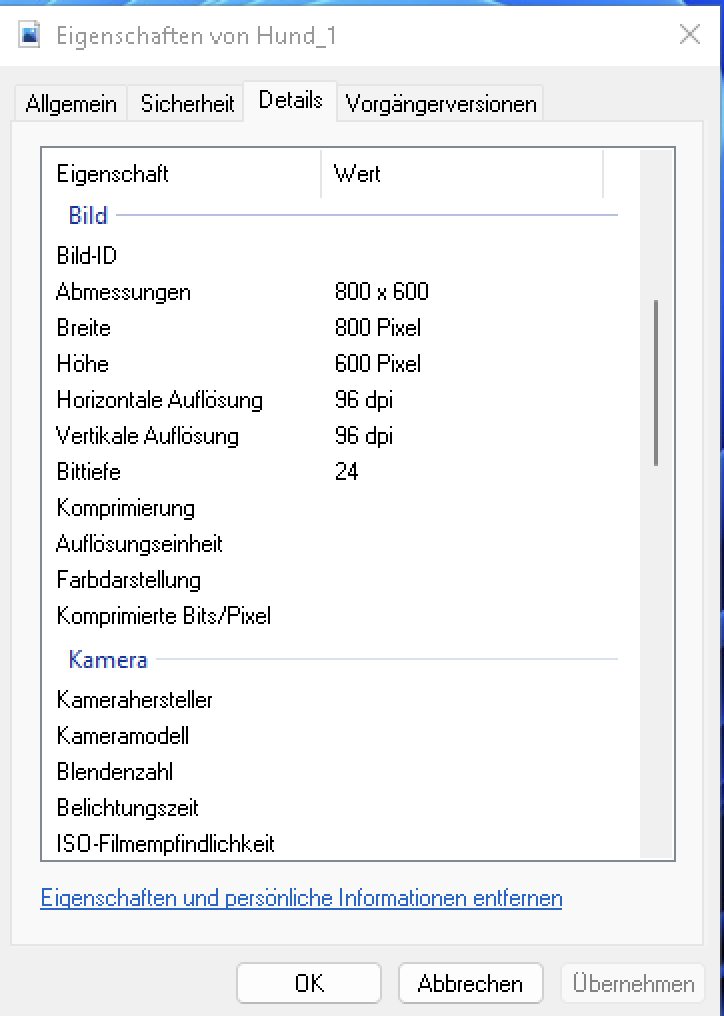
\includegraphics[scale=0.7]{Hund_1.png}
\end{minipage}
\begin{minipage}{0.49\linewidth}
	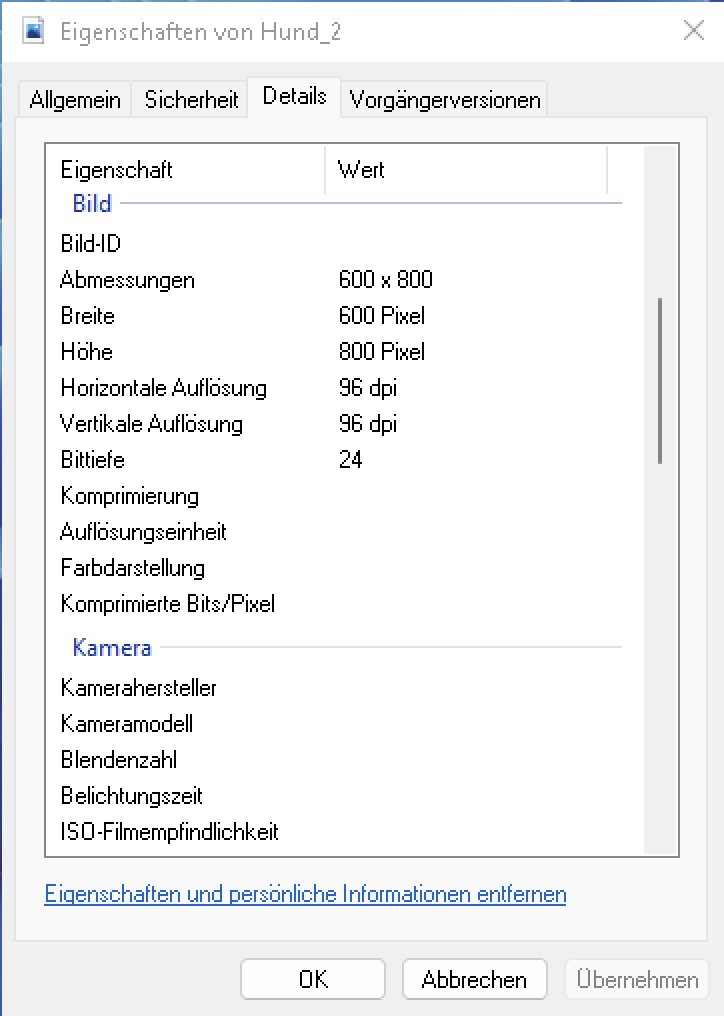
\includegraphics[scale=0.7]{Hund_2.png}
\end{minipage}
\vspace{1cm}
\begin{LKtext}
	Auflösung des Bildes "Hund\_1": \lk{800} x \lk{800} Pixel.
	
	Auflösung des Bildes "Hund\_2": \lk{800} x \lk{800} Pixel.
\end{LKtext}

\subsubsection*{Begründung:}
\liniert{4}


%\input
\label{LastPage}
\normalsize
\ifthenelse{\equal{\TYP}{Klassenarbeit}}{
\input{\patha/Erwartungsbild.tex}}
{}
\ifthenelse{\equal{\TYP}{Leistungskontrolle}}{
\input{\patha/Erwartungsbild.tex}}
{}


\end{document}